\documentclass[a4paper]{scrartcl}
%preambulo

\usepackage{fullpage}
\usepackage{lmodern}
\usepackage[spanish,activeacute]{babel}
\usepackage[T1]{fontenc}

\usepackage{xcolor}

\usepackage{graphicx}

\usepackage{minted}
\newcommand{\BashFancyFormatLine}{%
  \def\FancyVerbFormatLine##1{\$\,##1}%
}

\title{SSH\_SCP Y SFTP\_V01}
\author{Facundo Navarro}

\begin{document}

\maketitle

\section{SCP}
El comando \textit{scp} (secure copy) es un comando que permite copiar de forma segura y encriptada entre un sistema local y un sistema remoto, o entre dos sistemas remotos. Se pueden realizar las siguientes operaciones:
\begin{itemize}
	\item Copiar un archivo o directorio del sistema local a un sistema remoto.
	\item Copiar un archivo o directorio del sistema remoto a su sistema local.
	\item Copiar un archivo o directorio entre sistemas remotos desde su sistema local. 
\end{itemize}

La forma gen'erica del comando scp es:
\begin{minted}[formatcom=\BashFancyFormatLine]{bash}
ssh [-option] <origen> <destino>
\end{minted}

El comando \textit{scp} requiere autentificaci'on, se debe tener una cuenta o una clave p'ublica en el sistema de destino, y asegurarse de tener al menos permiso de lectura en el sistema de origen y permiso de escritura en el sistema de destino.

\subsection{Especificaciones del origen y el destino para la copia}
Se puede especificar el origen (el archivo o direcotorio que se copiar'a) y el destino (la ubicaci'on en la que se copiara el archivo o directorio). Por parte del cluster Navira, los directorios de destino se encuentran en \textit{/home/usuario}. Las siguientes secuencias para copiar un archivo \textit{"prueba.sh"} desde el sistema local hacia el remoto son equivalentes:

\begin{minted}[formatcom=\BashFancyFormatLine,breaklines]{bash}
scp -P 2230 /home/operador/prueba.sh fnavarro@navira.cidie.ucc.edu.ar:/home/fnavarro
scp -P 2230 $HOME/prueba.sh fnavarro@navira.cidie.ucc.edu.ar:/home/fnavarro
scp -P 2230 ~/prueba.sh fnavarro@navira.cidie.ucc.edu.ar:/home/fnavarro
scp -P 2230 prueba.sh fnavarro@navira.cidie.ucc.edu.ar:/home/fnavarro
\end{minted}

Los anteriores comandos de bash son equivalentes siempre y cuando \textit{"prueba.sh"} este en \textit{/home/operador} y el comando ssh se ejecute estando en dicho directorio, lo que expone que el car'acter de tilde \textcolor{blue}{\textasciitilde} y el alias \textit{\$HOME} representa el directorio \textit{home} del usuario logueado.

\begin{figure}[ht]
	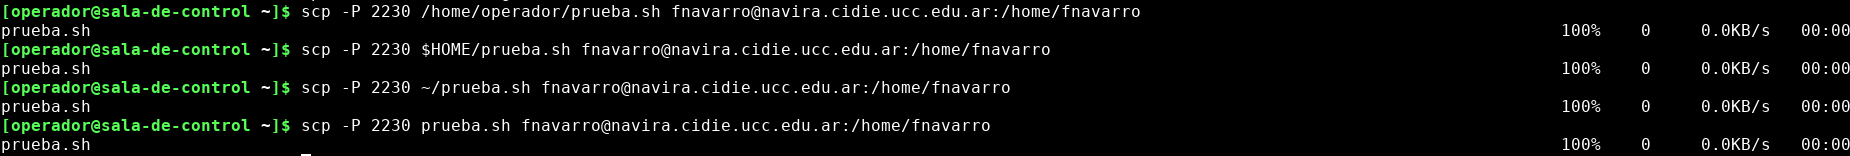
\includegraphics[width=\columnwidth]{./ssh_scp_sftp_imgs/samescp}
	\caption{Equivalencias de expresiones de PATH's}
	\label{fig:samescp}
\end{figure}

\subsection{Copiar archivos de LOCAL a SERVIDOR}
Si queremos copiar el archivo \textit{localfile.sh} de nuestro ordenador a la carpeta \textit{/home/usuario} del cluster, hacemos lo siguiente
\begin{minted}[formatcom=\BashFancyFormatLine,breaklines]{bash}
scp -P 2230 localfile.sh fnavarro@navira.cidie.ucc.edu.ar:/home/fnavarro
\end{minted}

\begin{figure}[ht]
	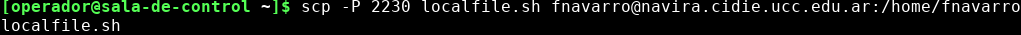
\includegraphics[width=\columnwidth]{./ssh_scp_sftp_imgs/LtoS}
	\caption{Copiando desde nuestro ordenador al Cluster}
	\label{fig:LtoS}
\end{figure}

\begin{figure}[ht]
	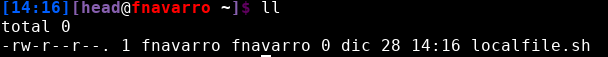
\includegraphics[scale=0.5]{./ssh_scp_sftp_imgs/LtoS_A}
	\caption{Archivo copiado en home del usuario fnavarro en el Cluster}
	\label{fig:LtoS_A}
\end{figure}

\subsection{Copiar de SERVIDOR a LOCAL}
Para traer archivos o directorios del Cluster hacia nuestro ordenador, como pueden ser los resultados de la ejecucion de los scripts. 
Para copiar un archivo \textit{.out} del Cluster hacia el directorio \textit{home} de nuestro ordenador se realiza de la siguiente manera:
\begin{minted}[formatcom=\BashFancyFormatLine,breaklines]{bash}
scp -P 2230 fnavarro@navira.cidie.ucc.edu.ar:/home/fnavarro/slurm-191.out $HOME
\end{minted}

\begin{figure}[!ht]
	
\includegraphics[width=\columnwidth]{./ssh_scp_sftp_imgs/StoL}
	\caption{Trayendo archivos desde el Cluster hacia nuestro ordenador}
	\label{fig:StoL}
\end{figure}

El mayor incoveniente de este m'etodo es tener que saber tanto el PATH completo del archivo o directorio que se quiere copiar como as'i tambi'en su nombre exacto, esto se facilita notablemente usando en vez de \textit{scp} el comando \textit{sftp} que se desarollar'a posteriormente.

\subsection{De SERVIDOR a otro SERVIDOR}
Generalizando
\begin{minted}[formatcom=\BashFancyFormatLine,breaklines]{bash}
scp user1@host1:/home/user1/foo1.txt user2@host2:/home/user2/foo2.txt 
\end{minted}

\subsection{Copia de directorios}
Los ejemplos vistos anteriormente hacen foco en la copia de archivos, pero tambi'en es posible copiar directorios enteros, tanto de servidor/local como local/servidor, agregando la opci'on:
\begin{description}
	\item[-r] se utiliza para realizar copias recursivas de directorios completos
\end{description}

\begin{minted}[formatcom=\BashFancyFormatLine,breaklines]{bash}
scp -P 2230 -r Documentos fnavarro@navira.cidie.ucc.edu.ar:/home/fnavarro
scp -P 2230 -r fnavarro@navira.cidie.ucc.edu.ar:/home/fnavarro/Resultados $HOME
\end{minted}

En la primer l'inea se env'ia la carpeta \textit{Documentos} al home del usuario fnavarro y en la segunda l'inea la carpeta \textit{Resultados} se copia al home del ordenador.


\section{SFTP}
SFTP es el acr'onimo para \textit{"Secure File Transfer Protocol"}, que no es m'as que el popular protocolo de comunicaci'on FTP con el agregado del cifrado que nos ofrece el protocolo SSH, creando una conexi'on segura con el servidor. Es de ventaja ya que el comando \textit{sftp}, una vez establecida el enlace, contiene una serie de comandos que permite navegar por los directorios tanto del servidor como del ordenador local.

En una primera medida se establece la conexi'on de manera similar a como se hace con \textit{ssh}.

\begin{minted}[formatcom=\BashFancyFormatLine,breaklines]{bash}
sftp -P 2230 fnavarro@navira.cidie.ucc.edu.ar
\end{minted}

Luego de garantizado el acceso, algunos de los comandos que se pueden ejecutar son:
\begin{description}
	\item[bye]	Sale de la sesi'on \textit{sftp}.
	\item[help]	Muestra todos los comandos\textit{sftp}.
	\item[ls]	Muestra los contenidos del directorio de trabajo remoto.
	\item[lls]	Muestra el contenido del directorio de trabajo local.
	\item[pwd]	Muestra el nombre del directorio de trabajo remoto.
	\item[cd]	Cambia el directorio de trabajo remoto.
	\item[lcd]	Cambia el directorio de trabajo local.
	\item[mkdir]	Crea un directorio en el sistema remoto.
	\item[lmkdir]	Crea un directorio en el sistema local.
	\item[rmdir]	Suprime un directorio en el sistma remoto
	\item[get]	Copia un archivo del directorio de trabajo remoto al local
	\item[put]	Copia un archivo del directorio de trabajo local al remoto
		
\end{description}

Como vemos en la imagen \ref{fig:sftp_1} primero nos logueamos al servidor, luego con \textit{ls -l} listamos los archivos que se encuentran en el \textit{home} del Cluster, y procedemos a copiar con el comando \textit{get} hacia el directorio donde estabamos posicionados antes de ejecutar \textit{sftp}
\begin{figure}[H]
	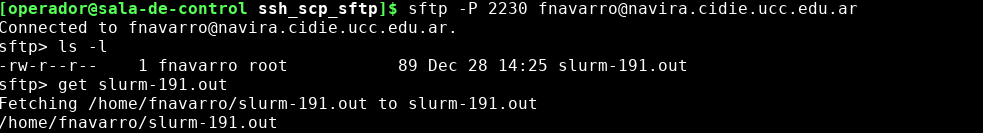
\includegraphics[width=\columnwidth]{./ssh_scp_sftp_imgs/sftp_1}
	\caption{Logueando a trav'es de sftp y copiando el archivo .out}
	\label{fig:sftp_1}
\end{figure}

Listando los archivos de mi directorio local a trav'es del comando \textit{lls -l} (local list), vemos que el archivo \textit{slurm-191.out} del Cluster se encuntra copiado en mi PC, como se ve en la figura \ref{fig:sftp_2}
\begin{figure}[!ht]
	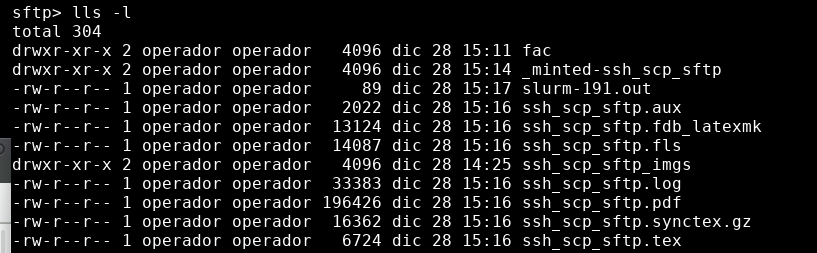
\includegraphics[width=\columnwidth]{./ssh_scp_sftp_imgs/sftp_2}
	\caption{Lista de archivos en directorio local}
	\label{fig:sftp_2}

\end{figure}

Ahora si queremos exportar al servidor el archivo \textit{ssh\_scp\_sftp.tex} hacemos lo que se observa en la imagen \ref{fig:sftp_3}
\begin{figure}[!ht]
	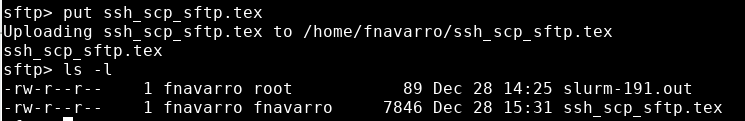
\includegraphics[width=\columnwidth]{./ssh_scp_sftp_imgs/sftp_3}
	\caption{Copiando en el Clusteri}
	\label{fig:sftp_3}
\end{figure}

Como comprobacion se listan los archivos y se ve que se encuentra el archivo \textit{.tex} que estaba en nuestro ordenador local.



\end{document}


